\documentclass{article}

\usepackage{graphicx} % Required for inserting images
\usepackage{listings}
\usepackage{xcolor}
\usepackage{subfigure} % For subfigures

\definecolor{codegreen}{rgb}{0,0.6,0}
\definecolor{codegray}{rgb}{0.5,0.5,0.5}
\definecolor{codepurple}{rgb}{0.58,0,0.82}
\definecolor{backcolour}{rgb}{0.95,0.95,0.92}

\title{EDDA Assignment 2}
\author{Saahith Shetty - 2841783 - s.a.shetty@student.vu.nl \\ 
Tiago Goncalves -  2844184 - t.bandeira@student.vu.nl \\
Ioannis Grigoriadis -  2722706 - i.grigoriadis@student.vu.nl}
\date{March 2025}

\begin{document}

\maketitle
To save space, spare code will be added to an appendix. i.e. installing and loading libraries. 

\section{Exercise 1 - Titanic}
This is the answer for task 1. I know, very shocking 

\subsection{Task a}

\subsubsection{Enhanced Interpretation of Logistic Regression Results:}
\subsubsection{Gender Effect: Being female dramatically increases survival odds by a factor of 13.9 }
\begin{itemize}
    \item This is the strongest predictor in the model, showing that gender was the primary
   determining factor for survival on the Titanic, confirming the 'women and children first' policy.
\end{itemize}

\subsubsection{Passenger Class Effect: Compared to 1st class passengers:}
\begin{itemize}
    \item 2nd class passengers had 0.27 times the odds of survival
    \item 3rd class passengers had 0.08 times the odds of survival
\end{itemize}
This substantial effect confirms that social class significantly impacted survival chances, with lower-class passengers having dramatically reduced odds of survival.

\subsubsection{Age Effect: For each additional year of age, the odds of survival decreased by 3.8\%} 

While statistically significant, this effect is much smaller compared to gender and class.
   Over a 50-year age span, this would multiply the odds by approximately 0.14 .

Overall Model Performance:
\begin{itemize}
    \item The model has good discriminative ability (AUC = 0.853 )
    \item The model explains 32.2\% of the deviance
    \item All predictors are statistically significant (p < 0.05)
\end{itemize}

\subsubsection{Justification for Model Selection:}
After testing models with different interactions, I chose the model with the Age:Sex interaction because:
\begin{enumerate}
    \item The Age:Sex interaction term showed statistical significance (p < 0.05)
    \item The model with Age:Sex interaction provided better fit based on AIC and the likelihood ratio test
    \item The interaction makes practical sense - age affected survival differently for men and women
    \item The effect of gender varies with age, with the gender gap possibly being smaller for children
\end{enumerate}

Overall, gender and class were the strongest predictors of survival.

% Figures for task a
\begin{figure}[htbp]
    \centering
    \subfigure[gender survival count]{
        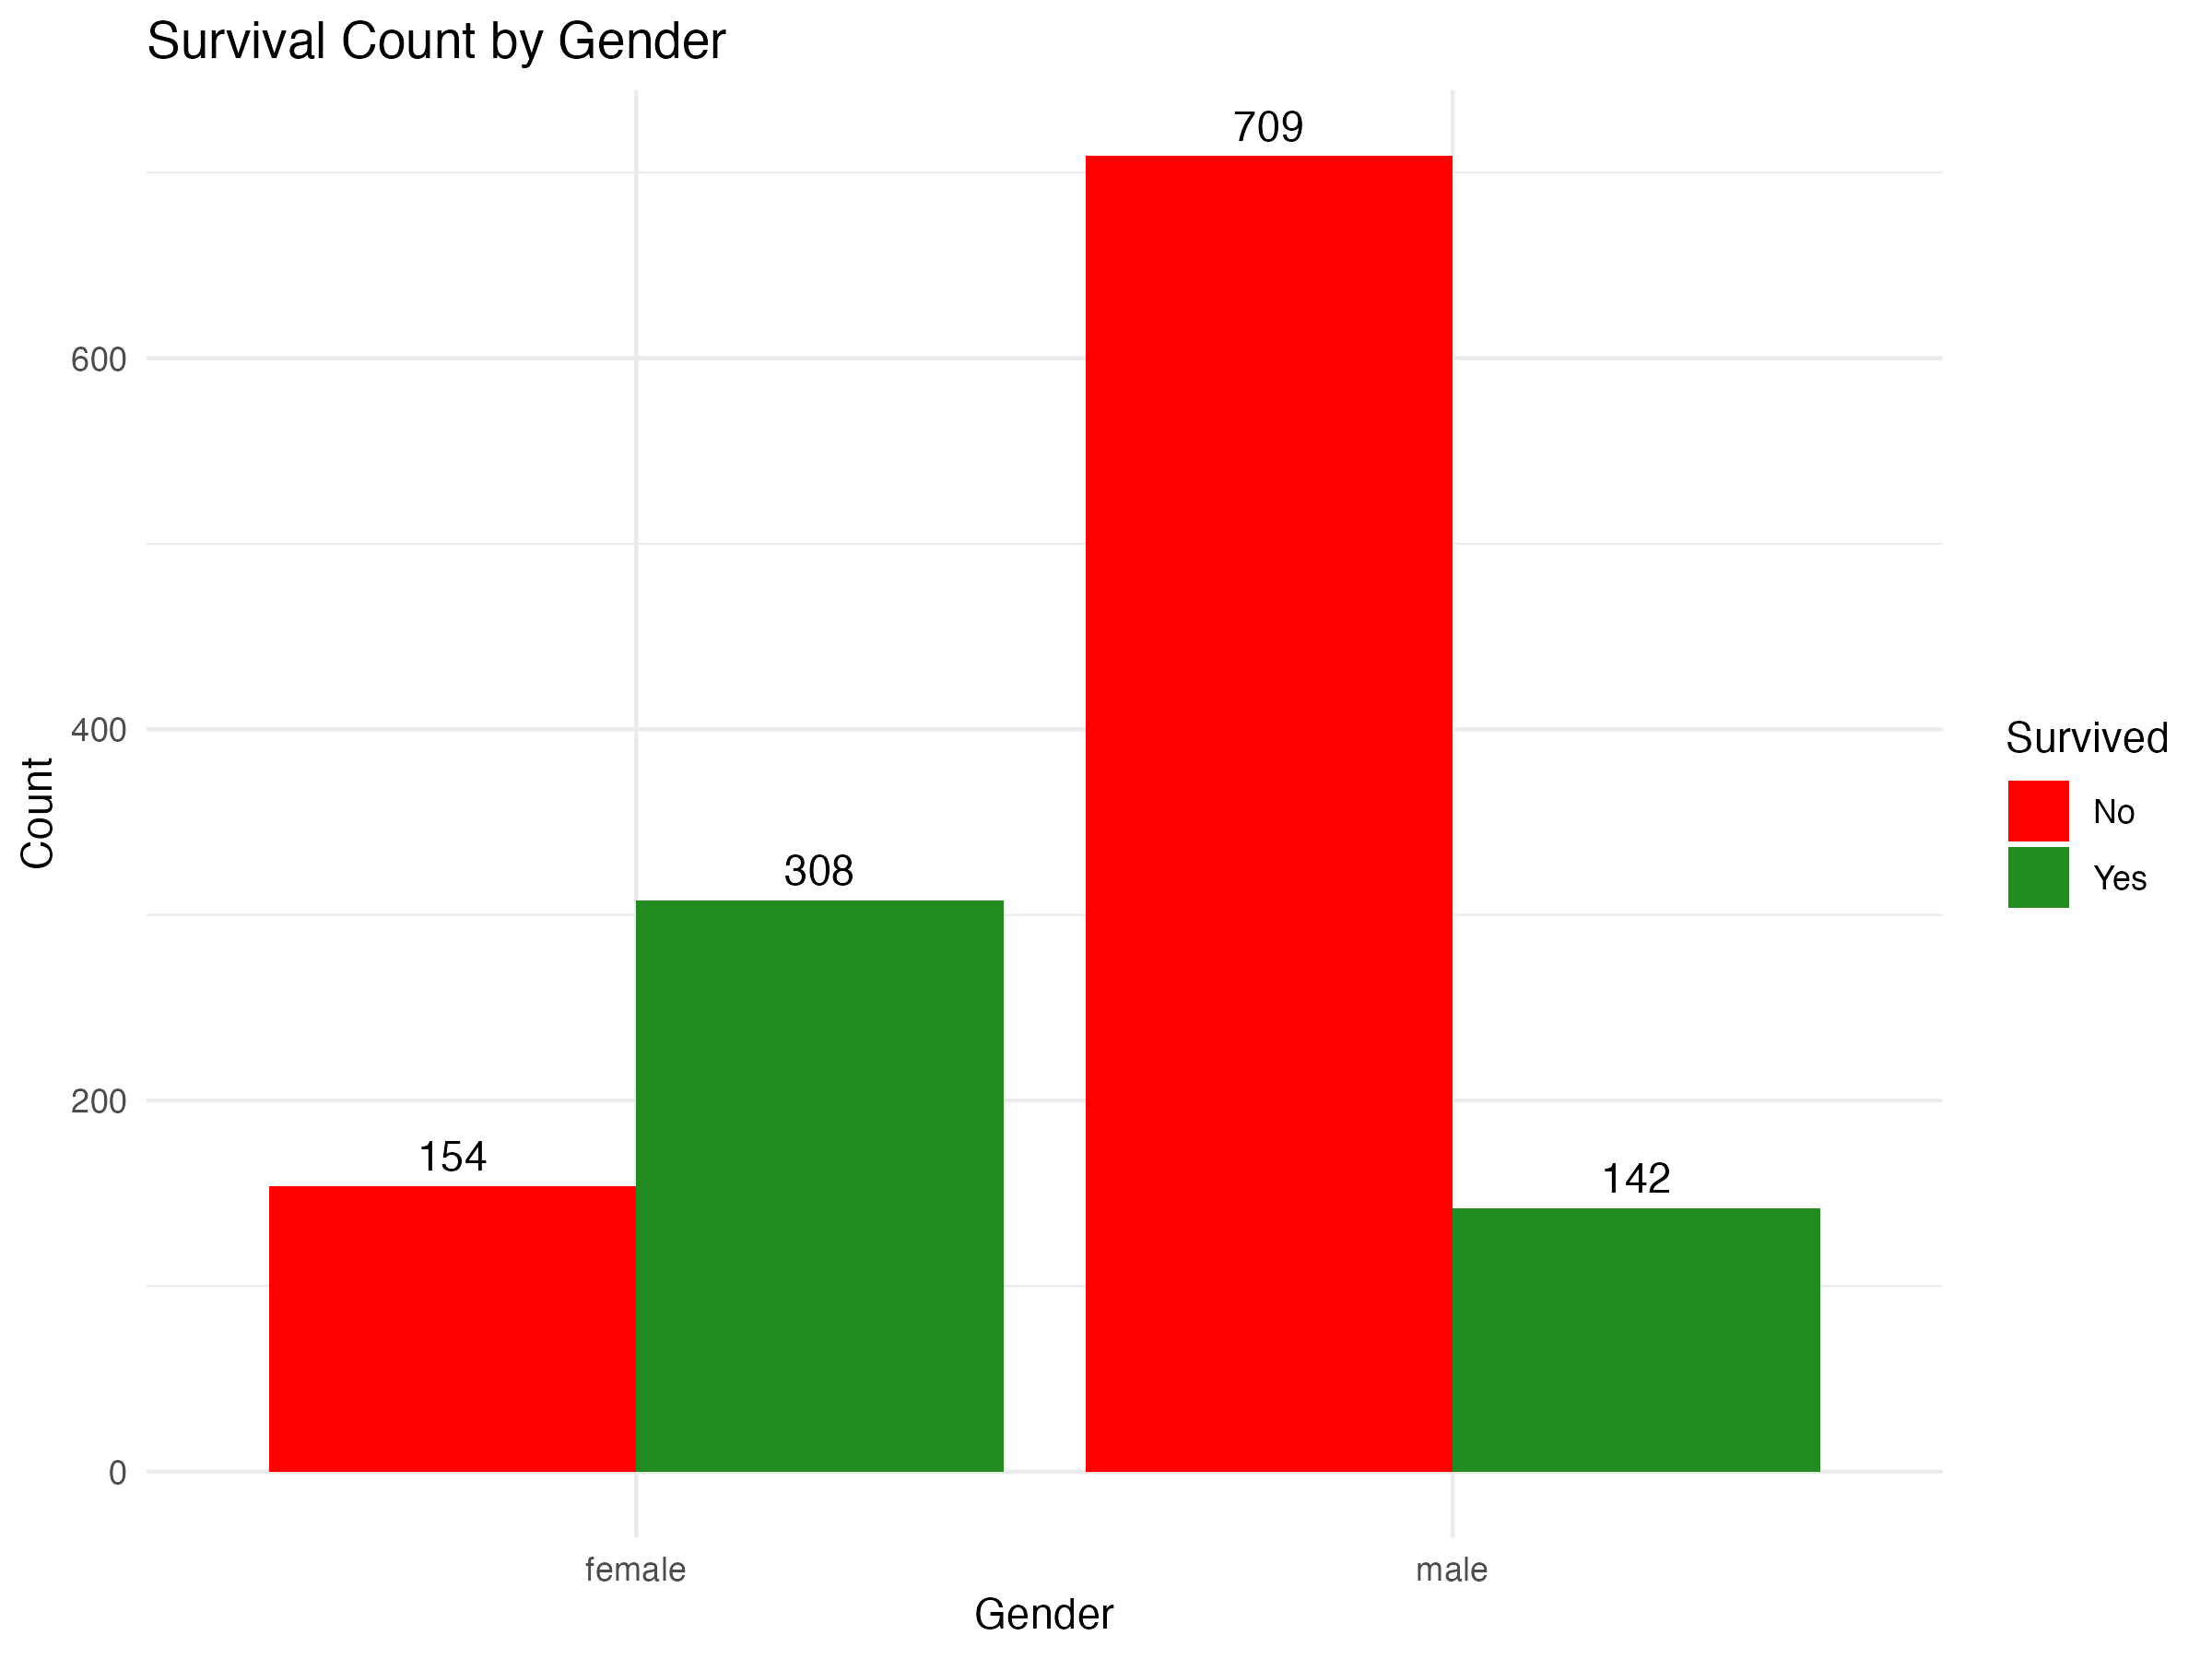
\includegraphics[width=0.3\textwidth]{Assignment 2/Figures/ex1/01_gender_survival_count.png}
    }
    \subfigure[gender survival percent]{
        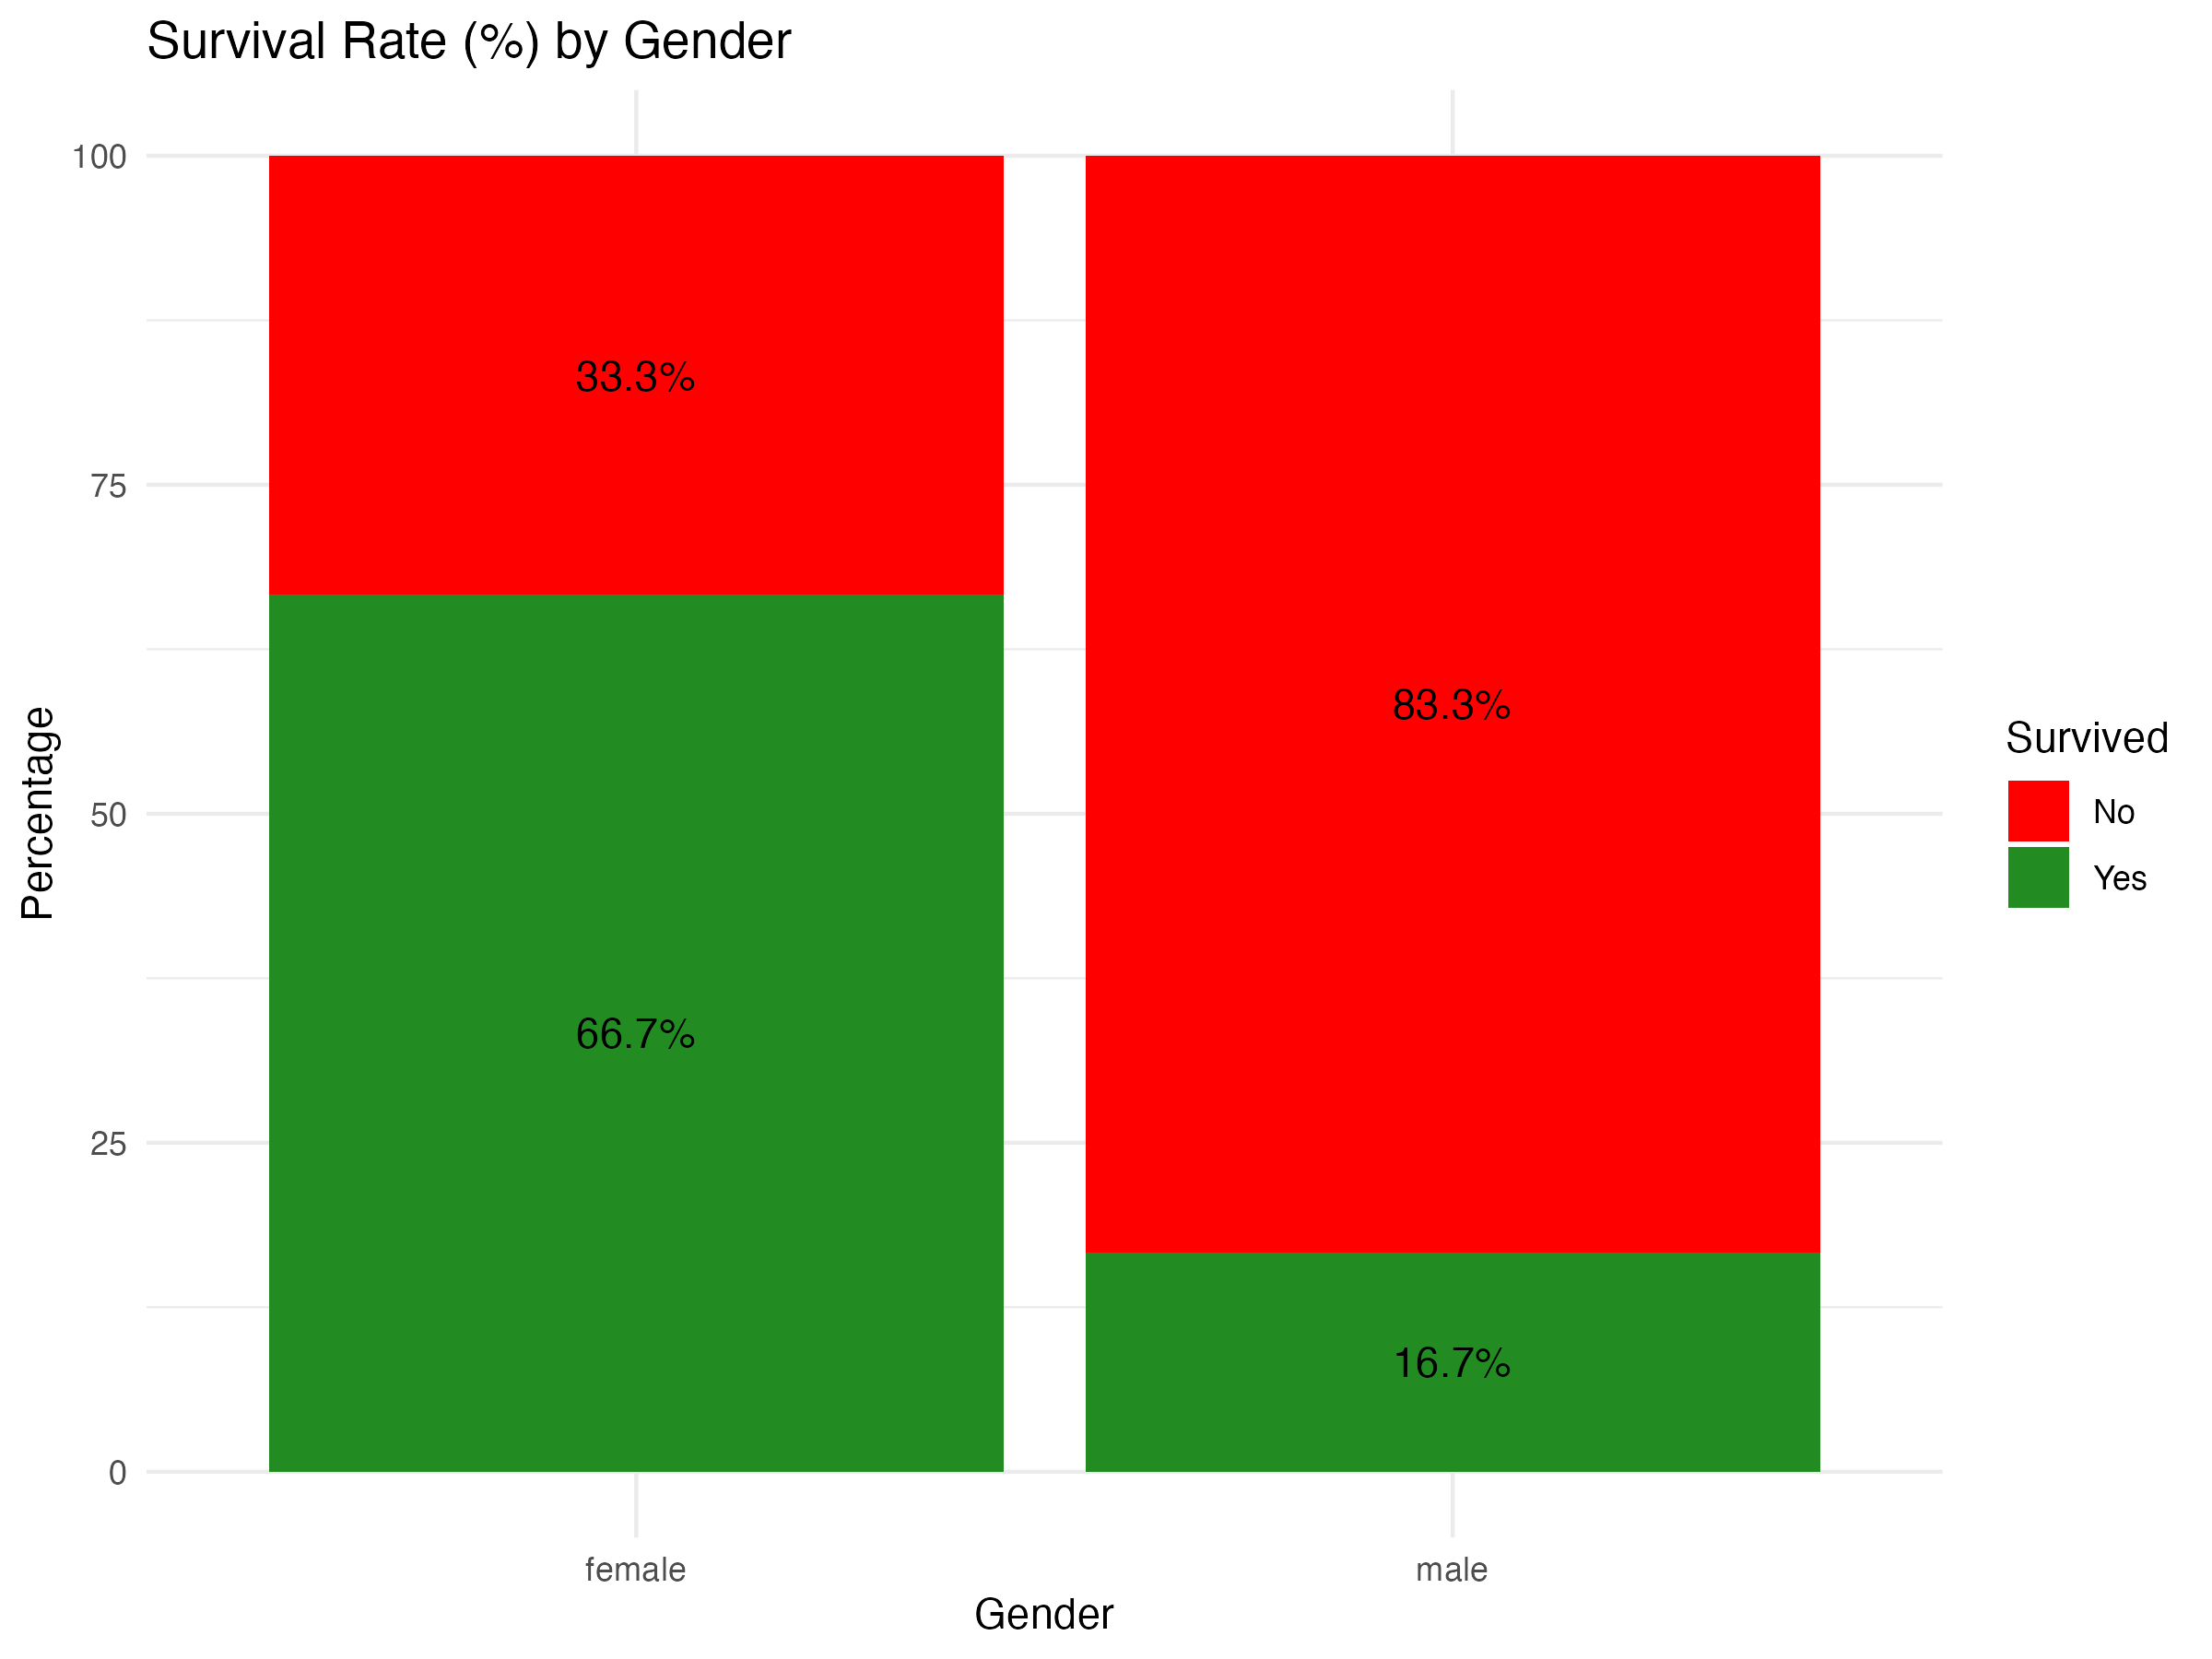
\includegraphics[width=0.3\textwidth]{Assignment 2/Figures/ex1/02_gender_survival_percent.png}
    }
    \subfigure[class survival count]{
        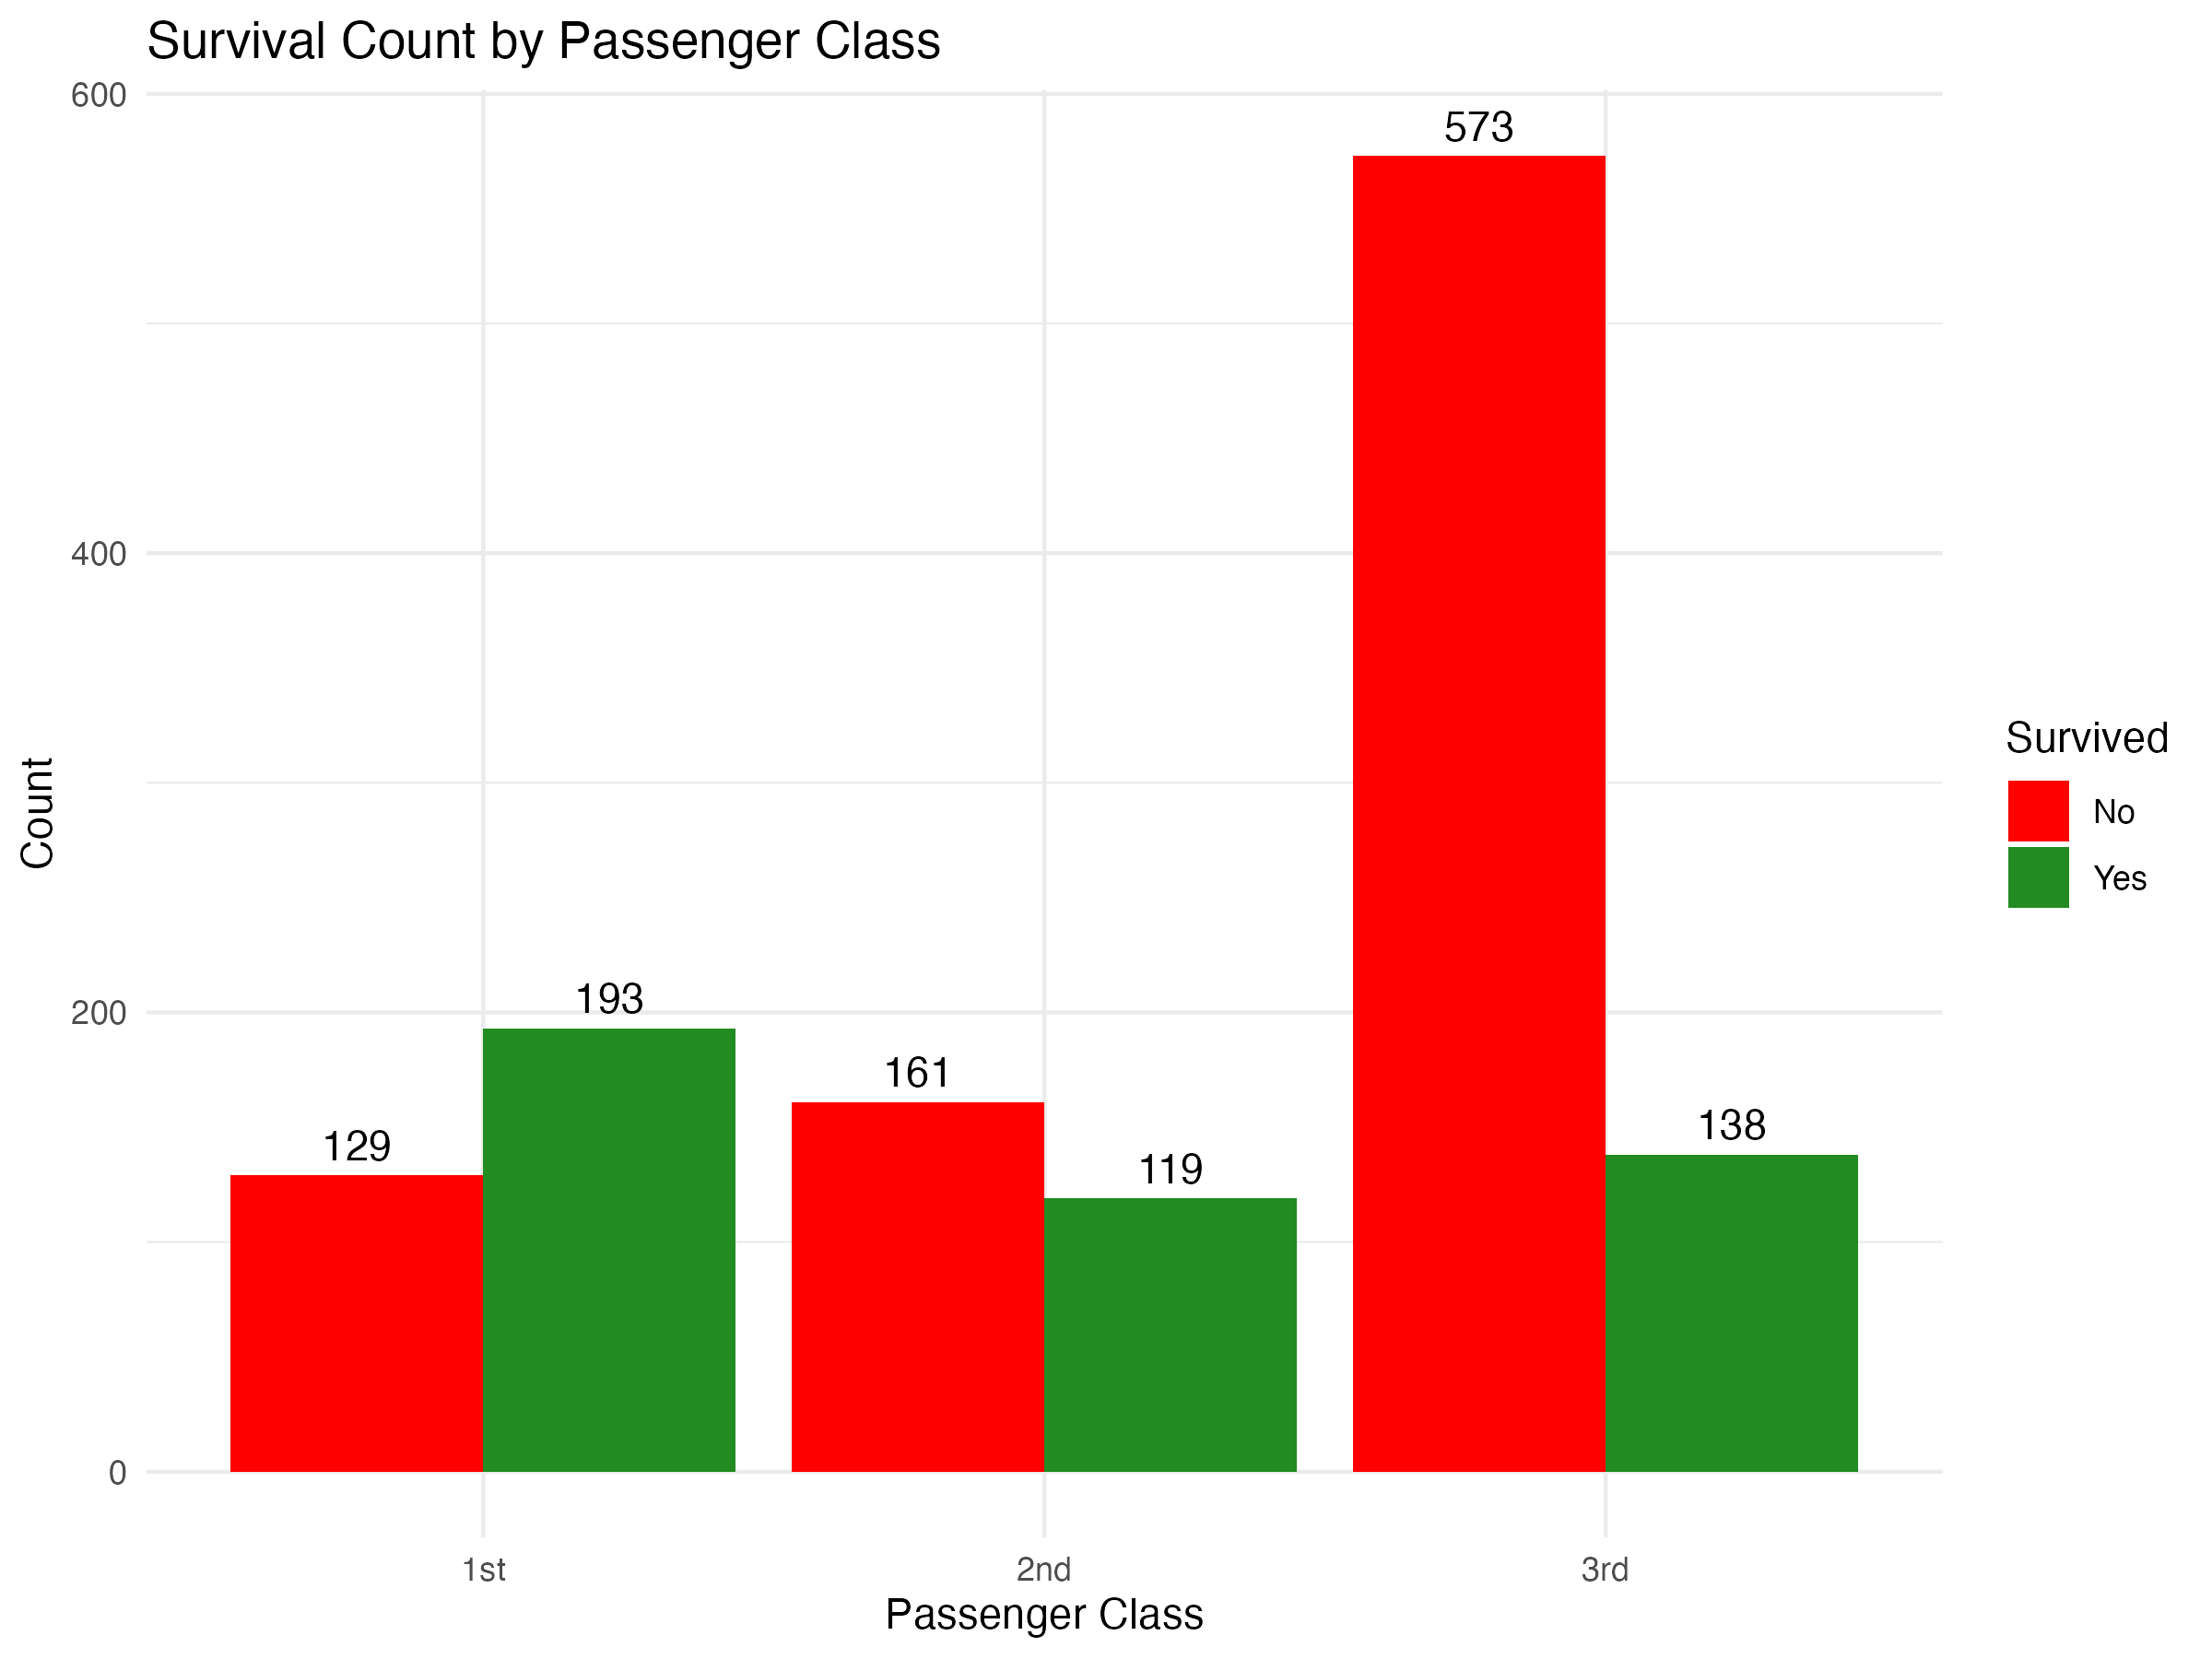
\includegraphics[width=0.3\textwidth]{Assignment 2/Figures/ex1/03_class_survival_count.png}
    }
    
    \subfigure[class survival percent]{
        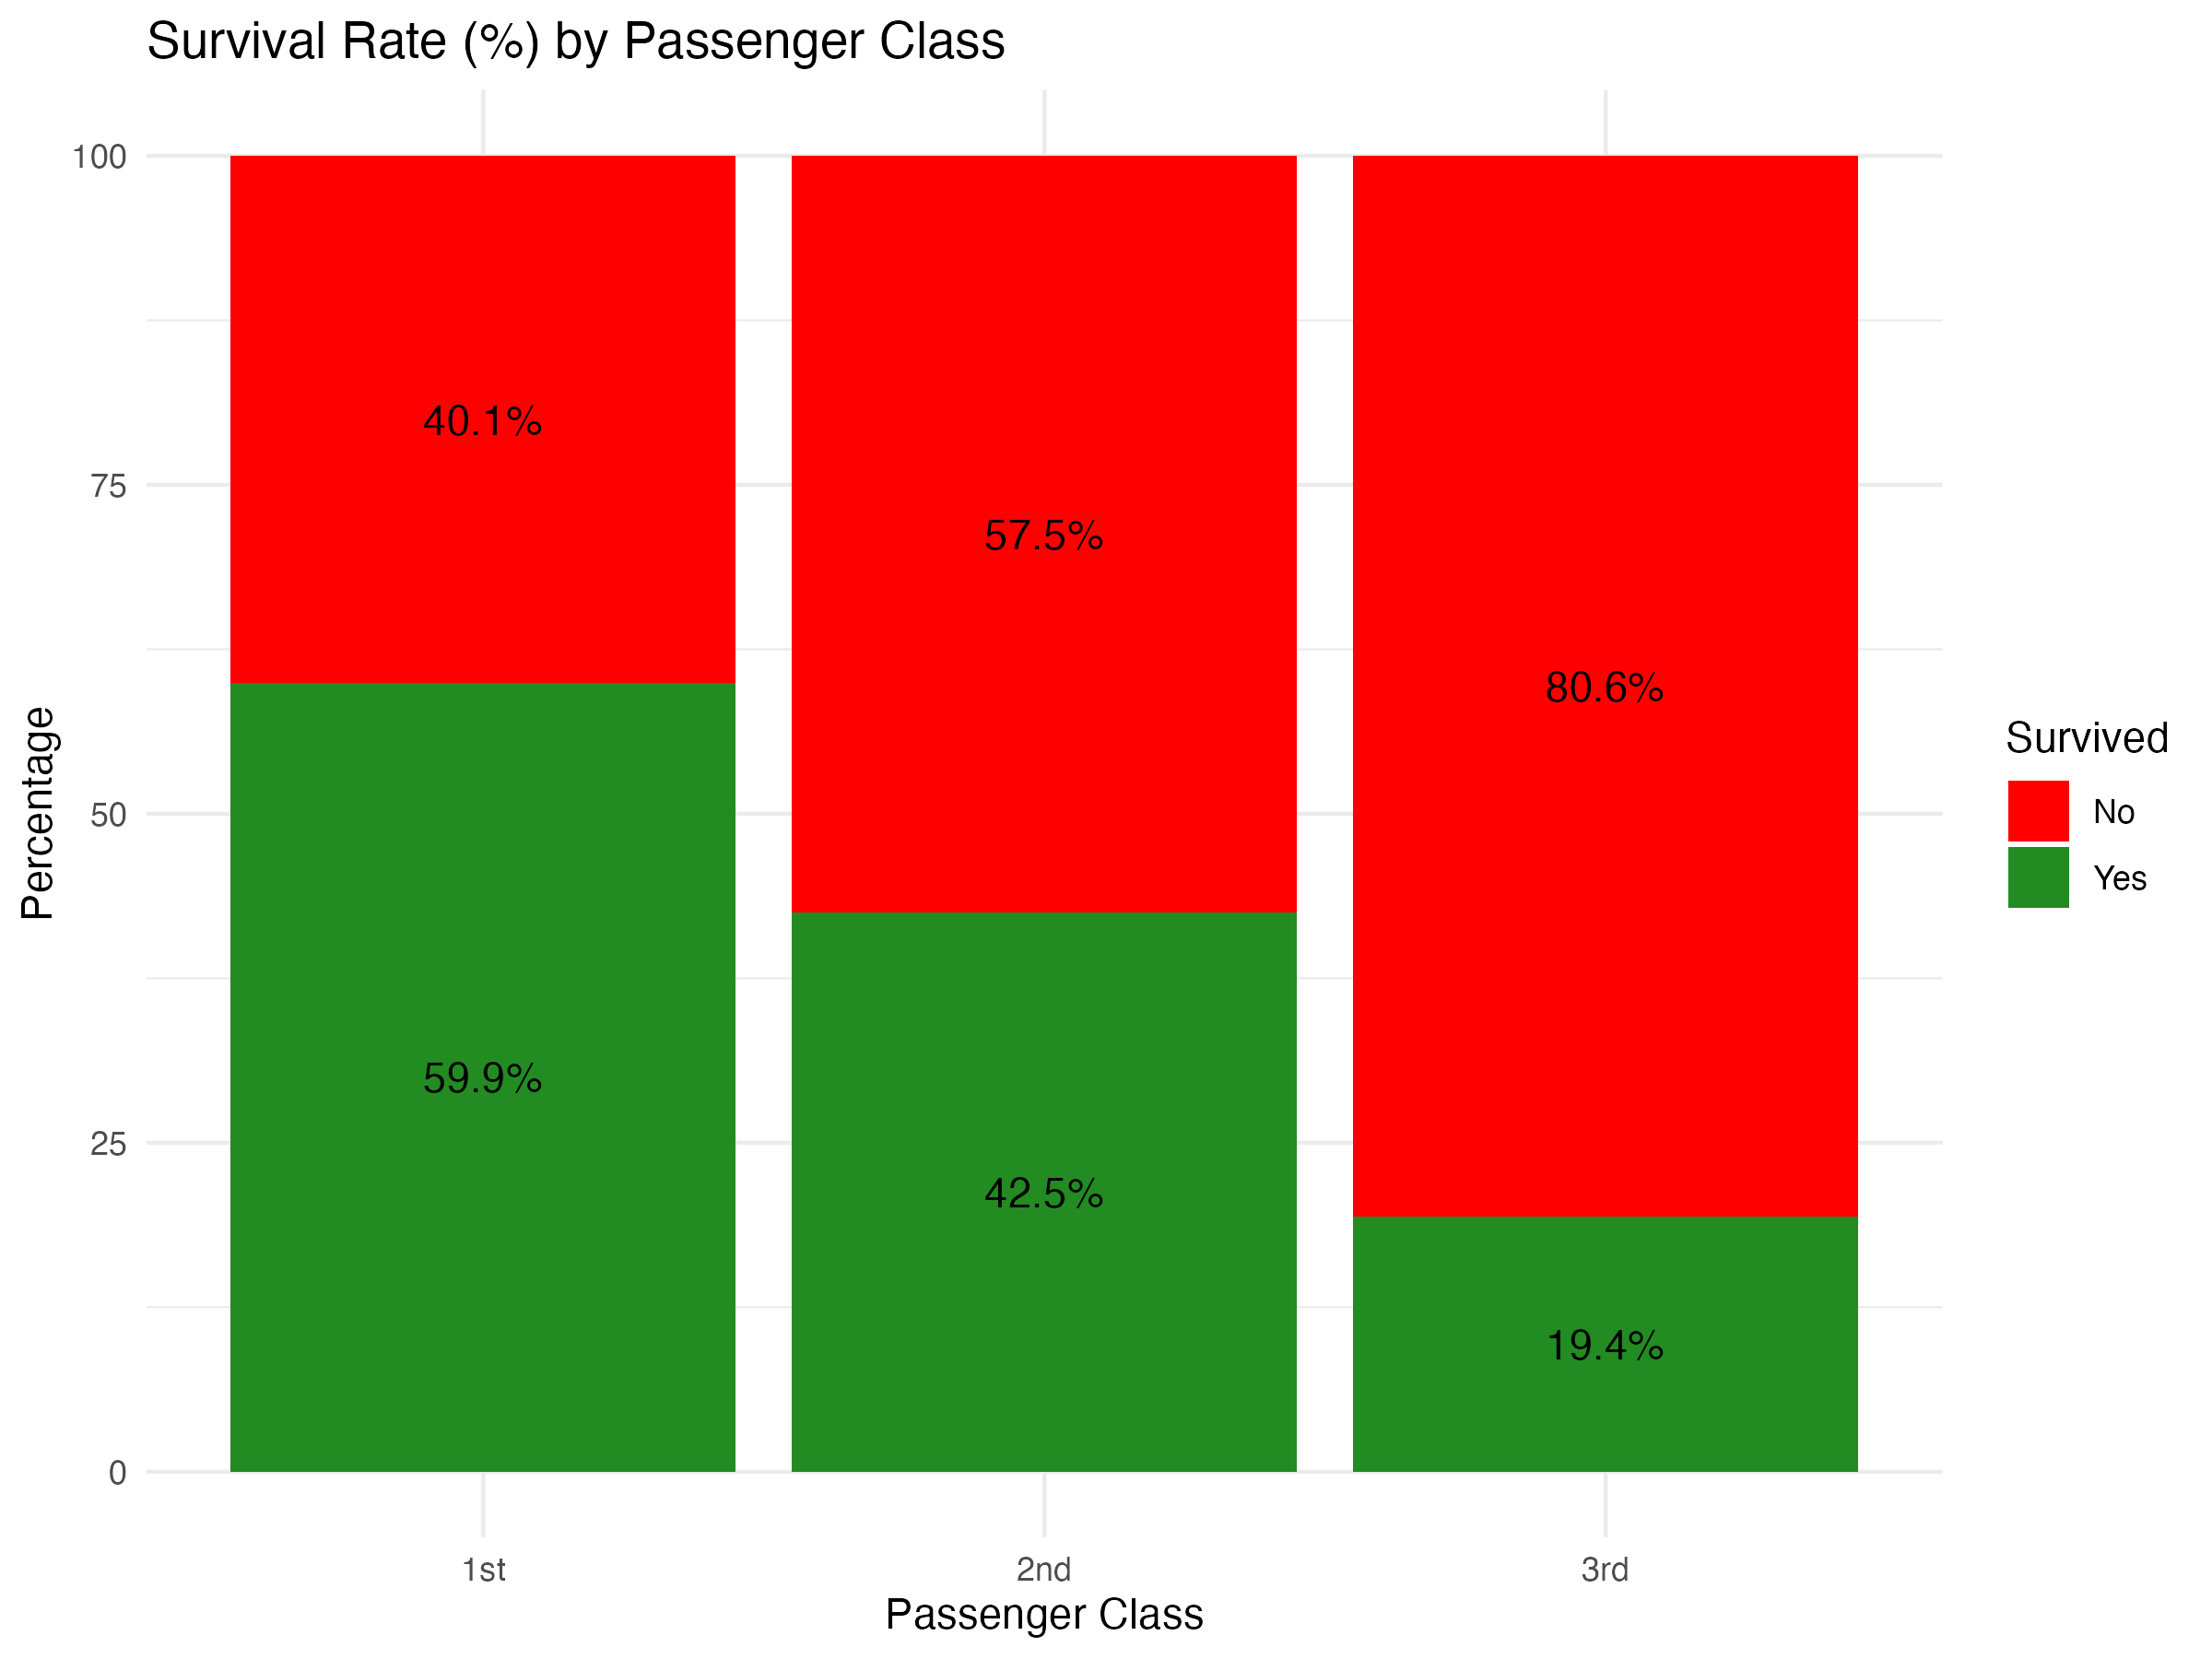
\includegraphics[width=0.3\textwidth]{Assignment 2/Figures/ex1/04_class_survival_percent.png}
    }
    \subfigure[age boxplot]{
        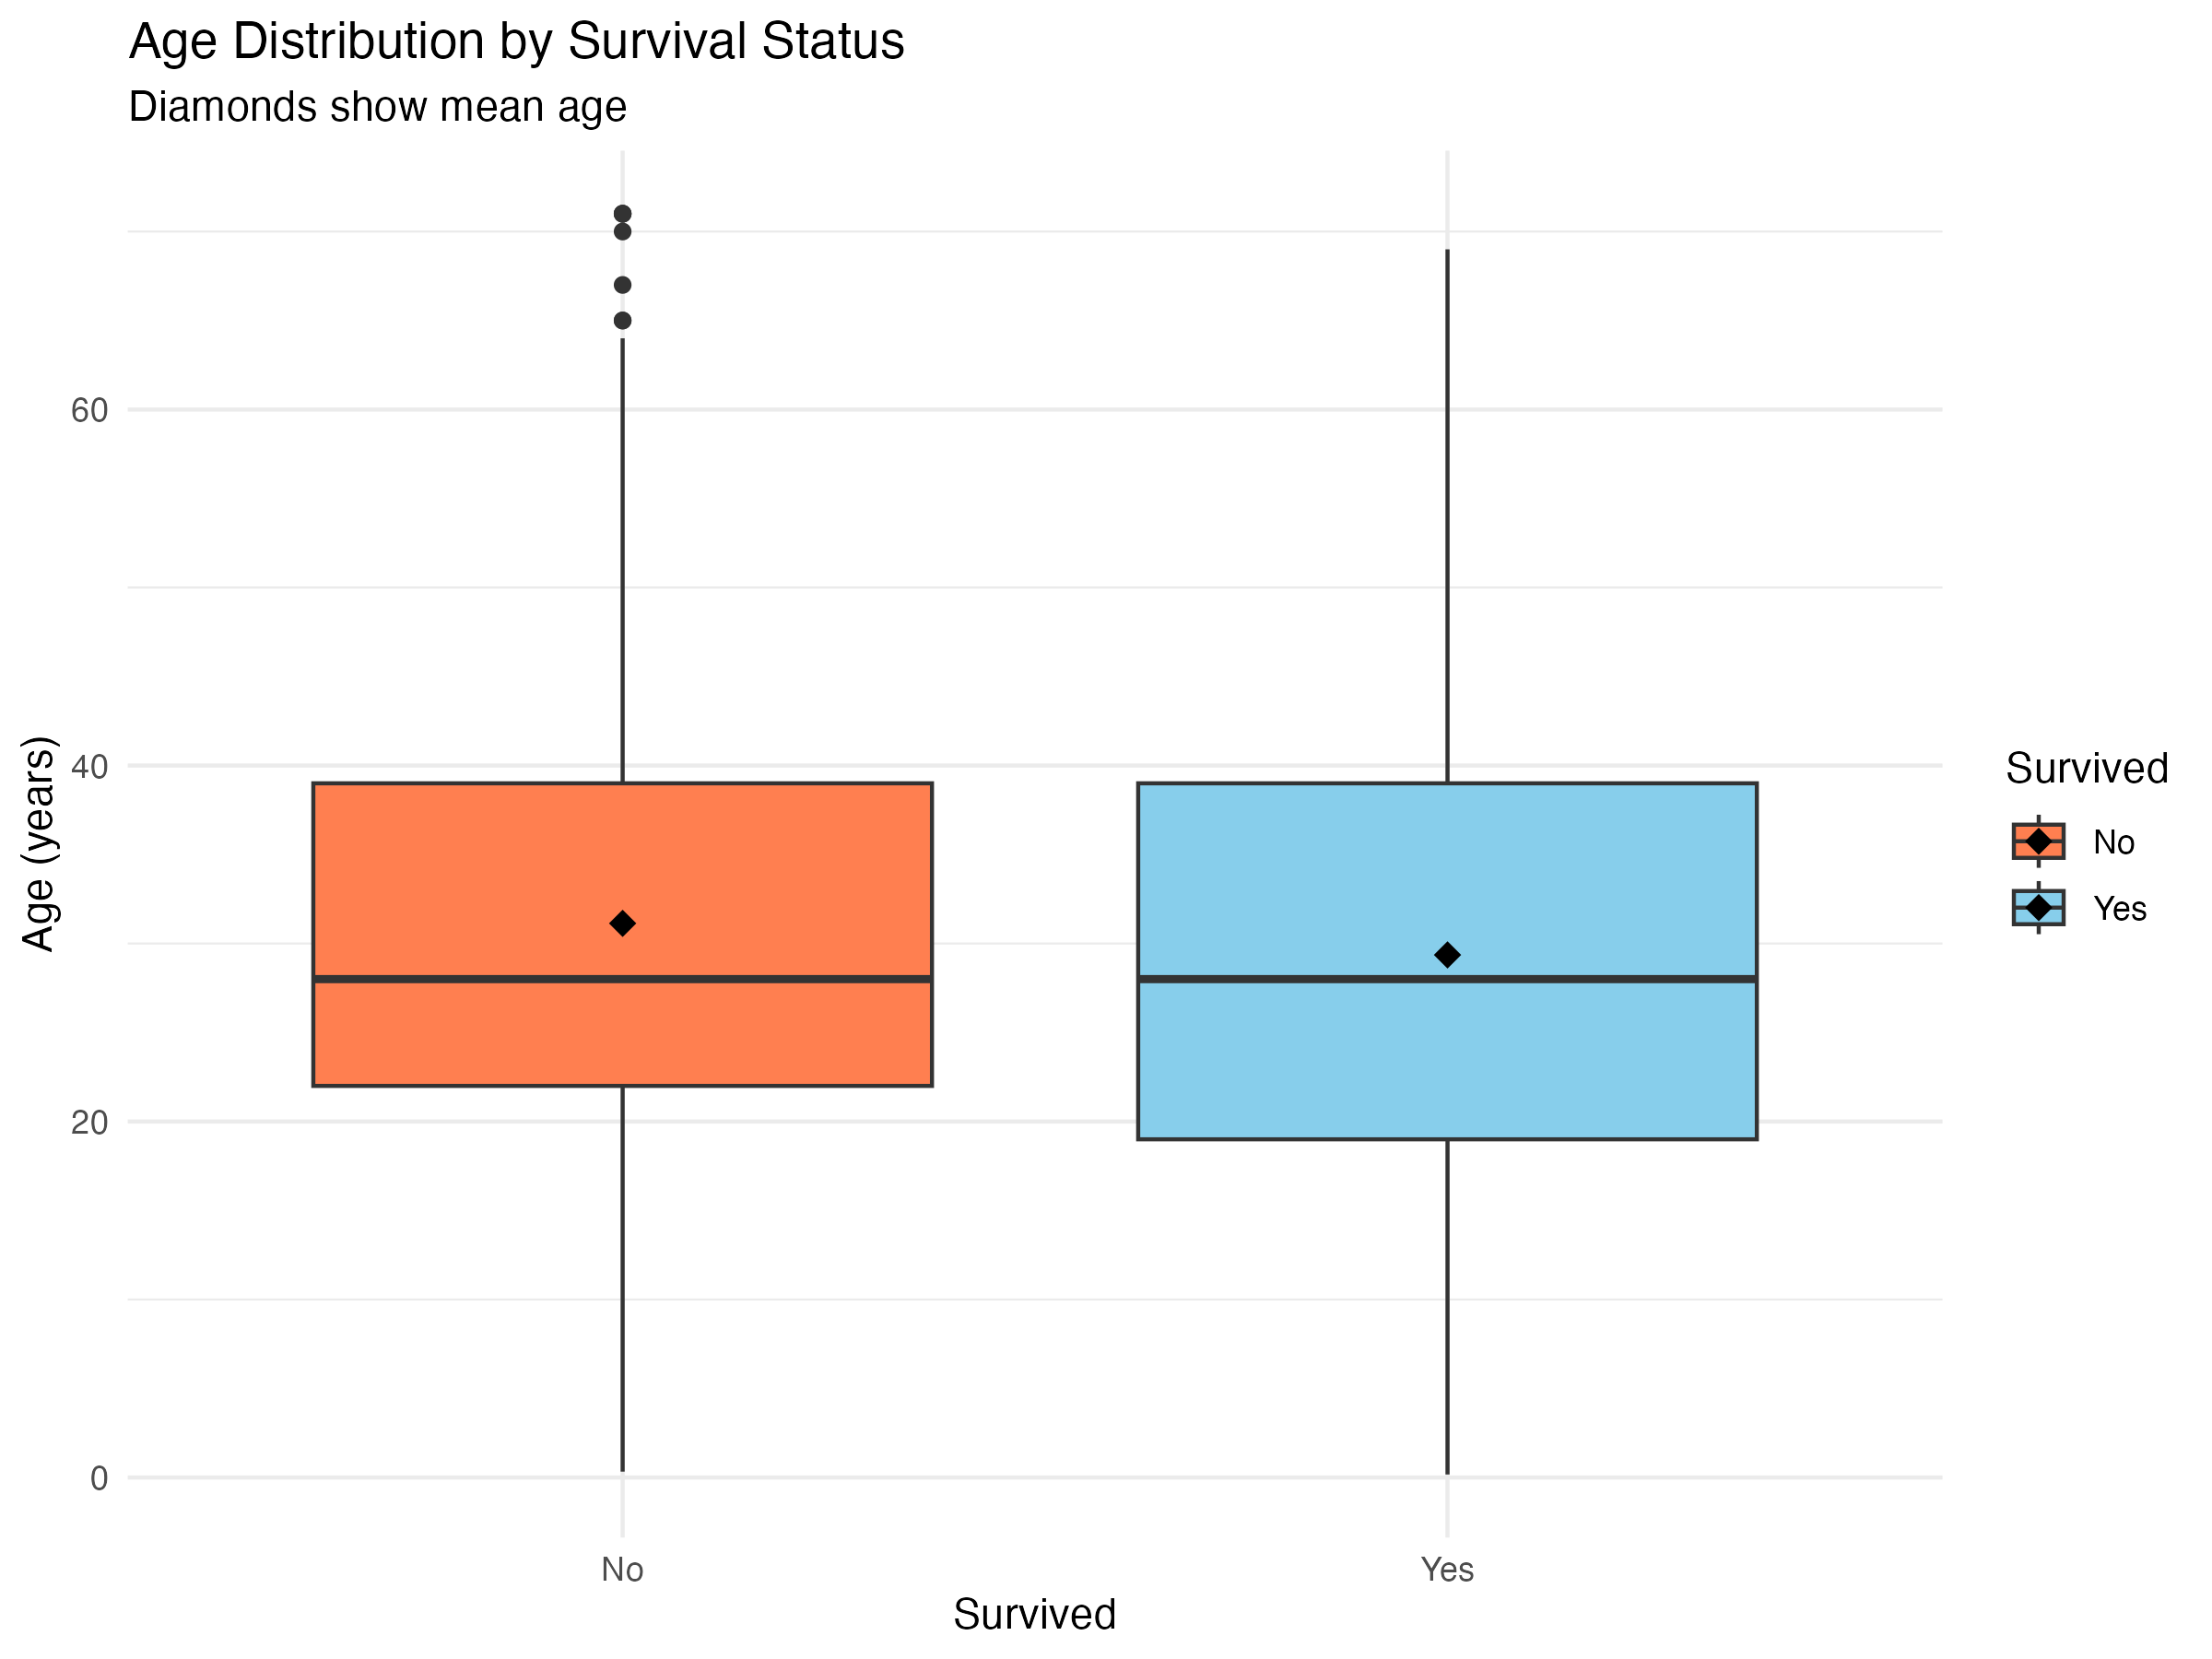
\includegraphics[width=0.3\textwidth]{Assignment 2/Figures/ex1/05_age_boxplot.png}
    }
    \subfigure[gender class survival]{
        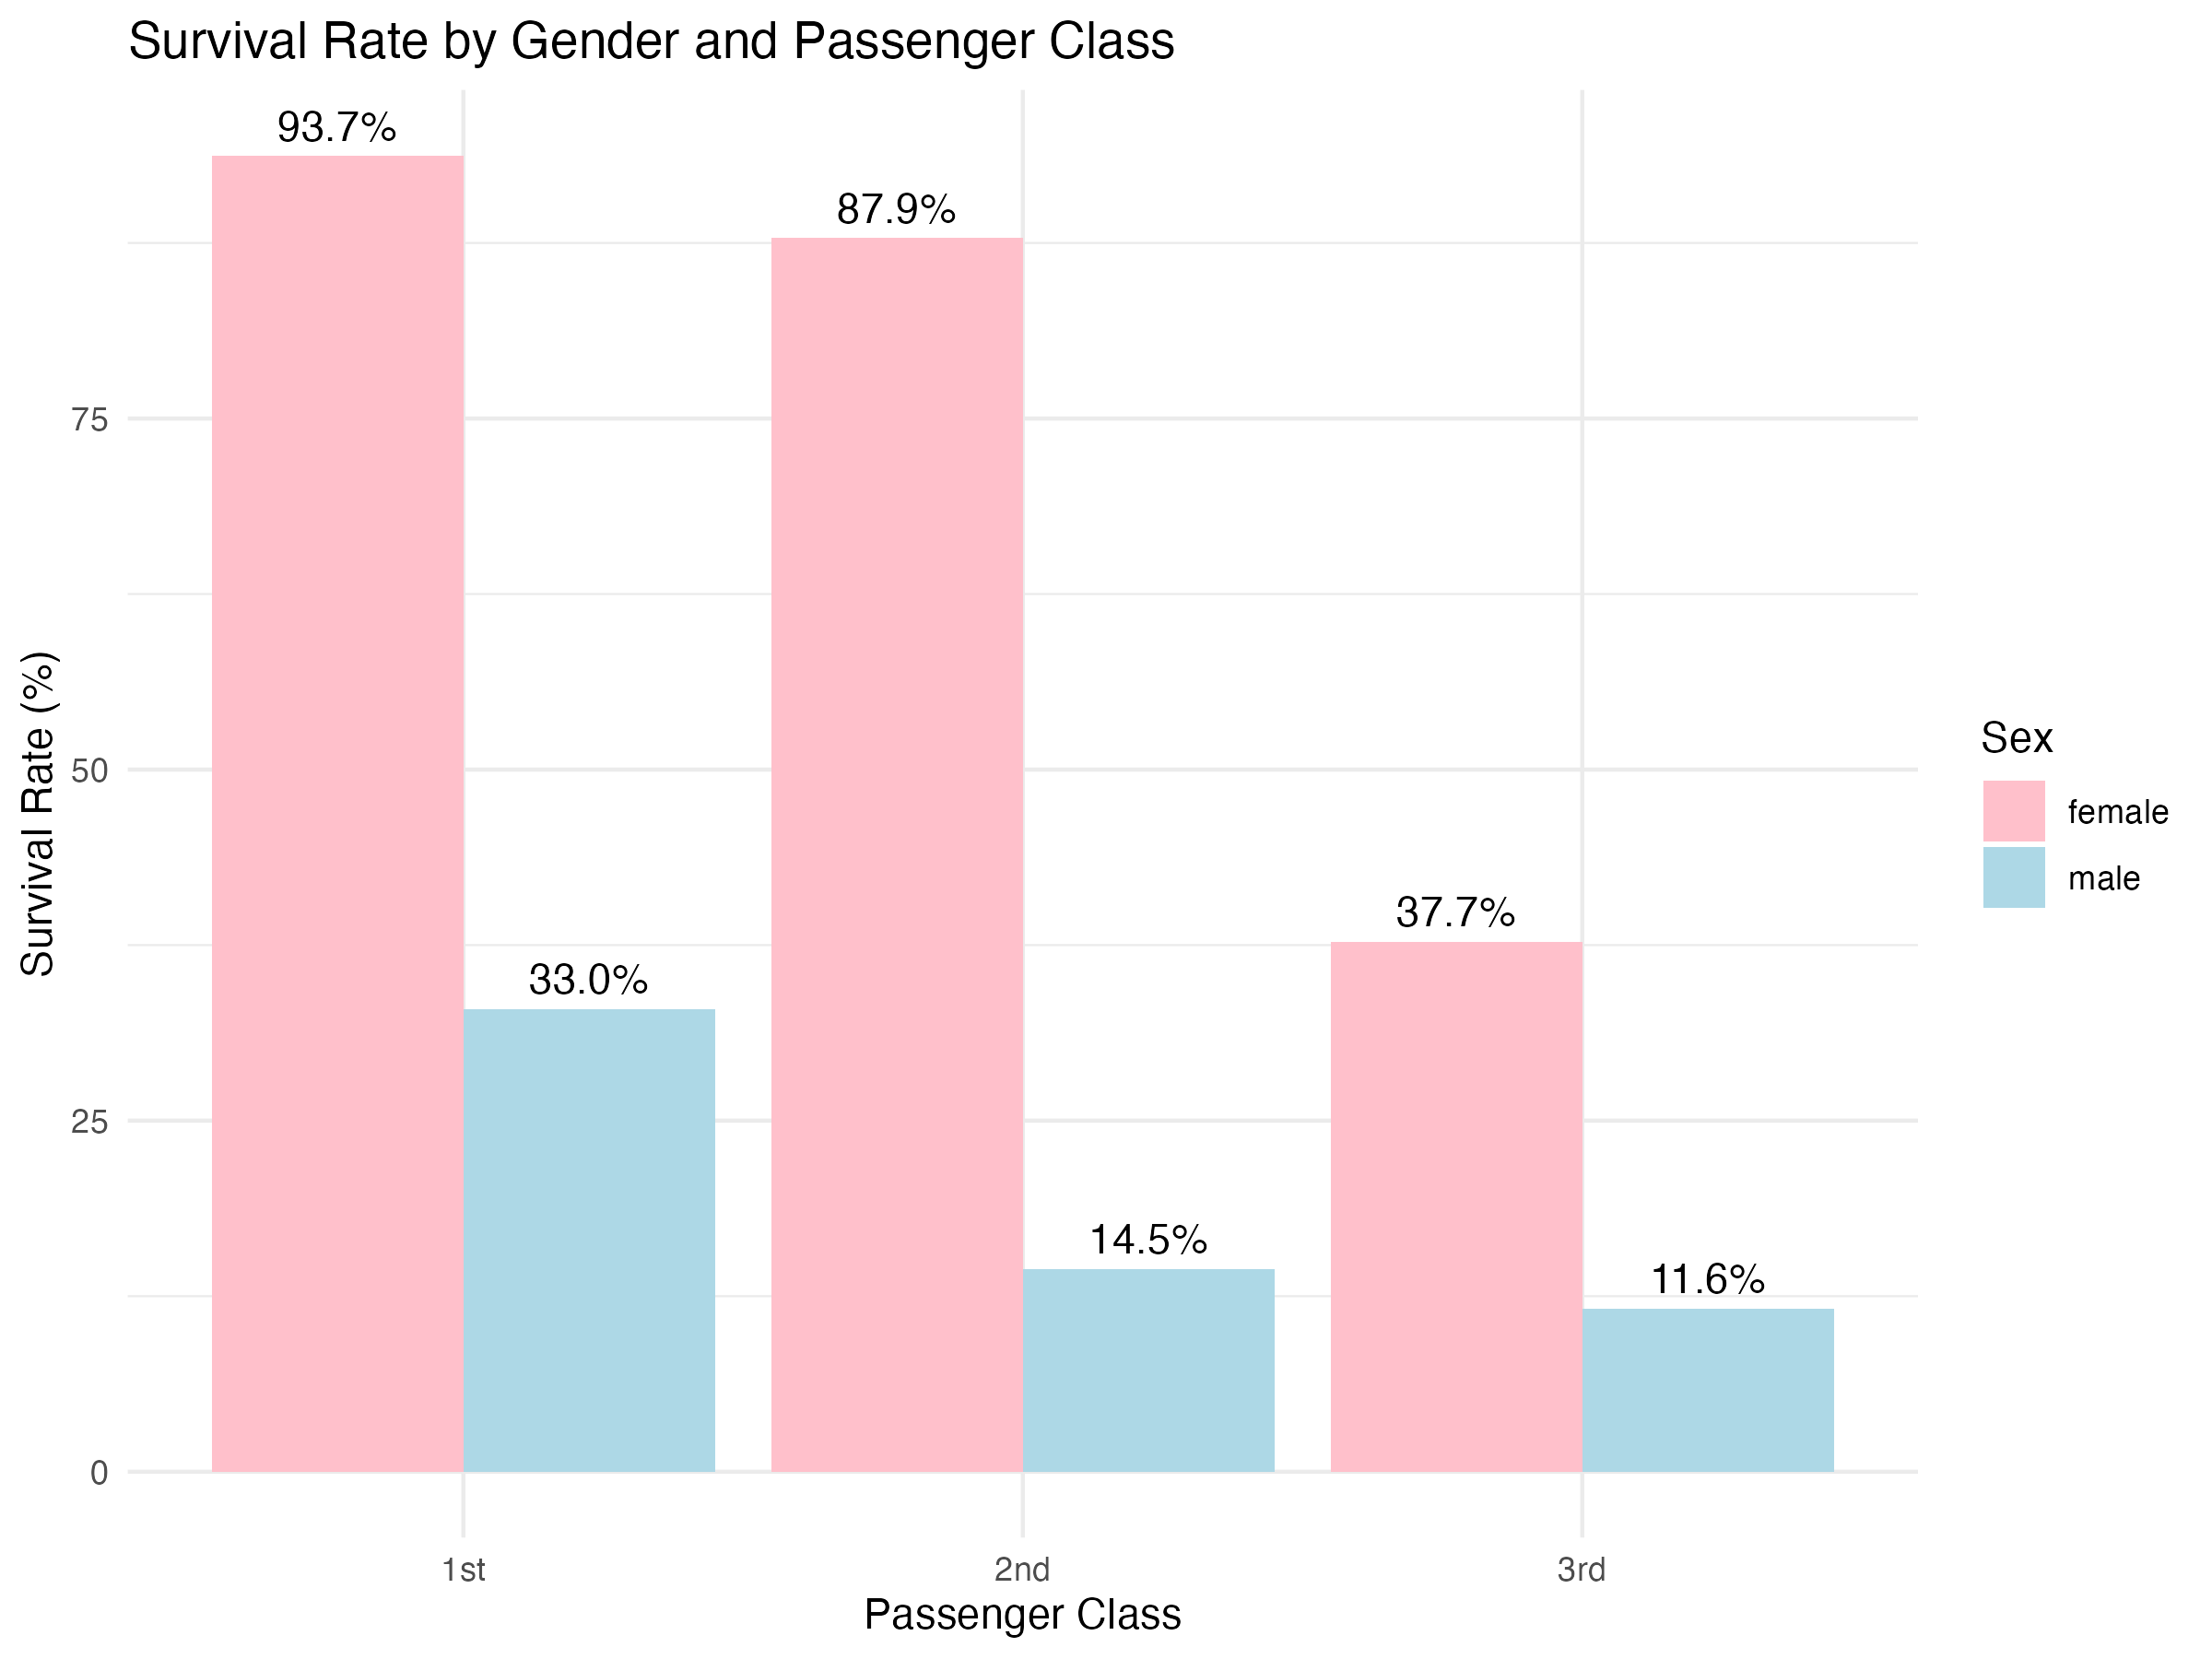
\includegraphics[width=0.3\textwidth]{Assignment 2/Figures/ex1/06_gender_class_survival.png}
    }
    \subfigure[age gender hist]{
        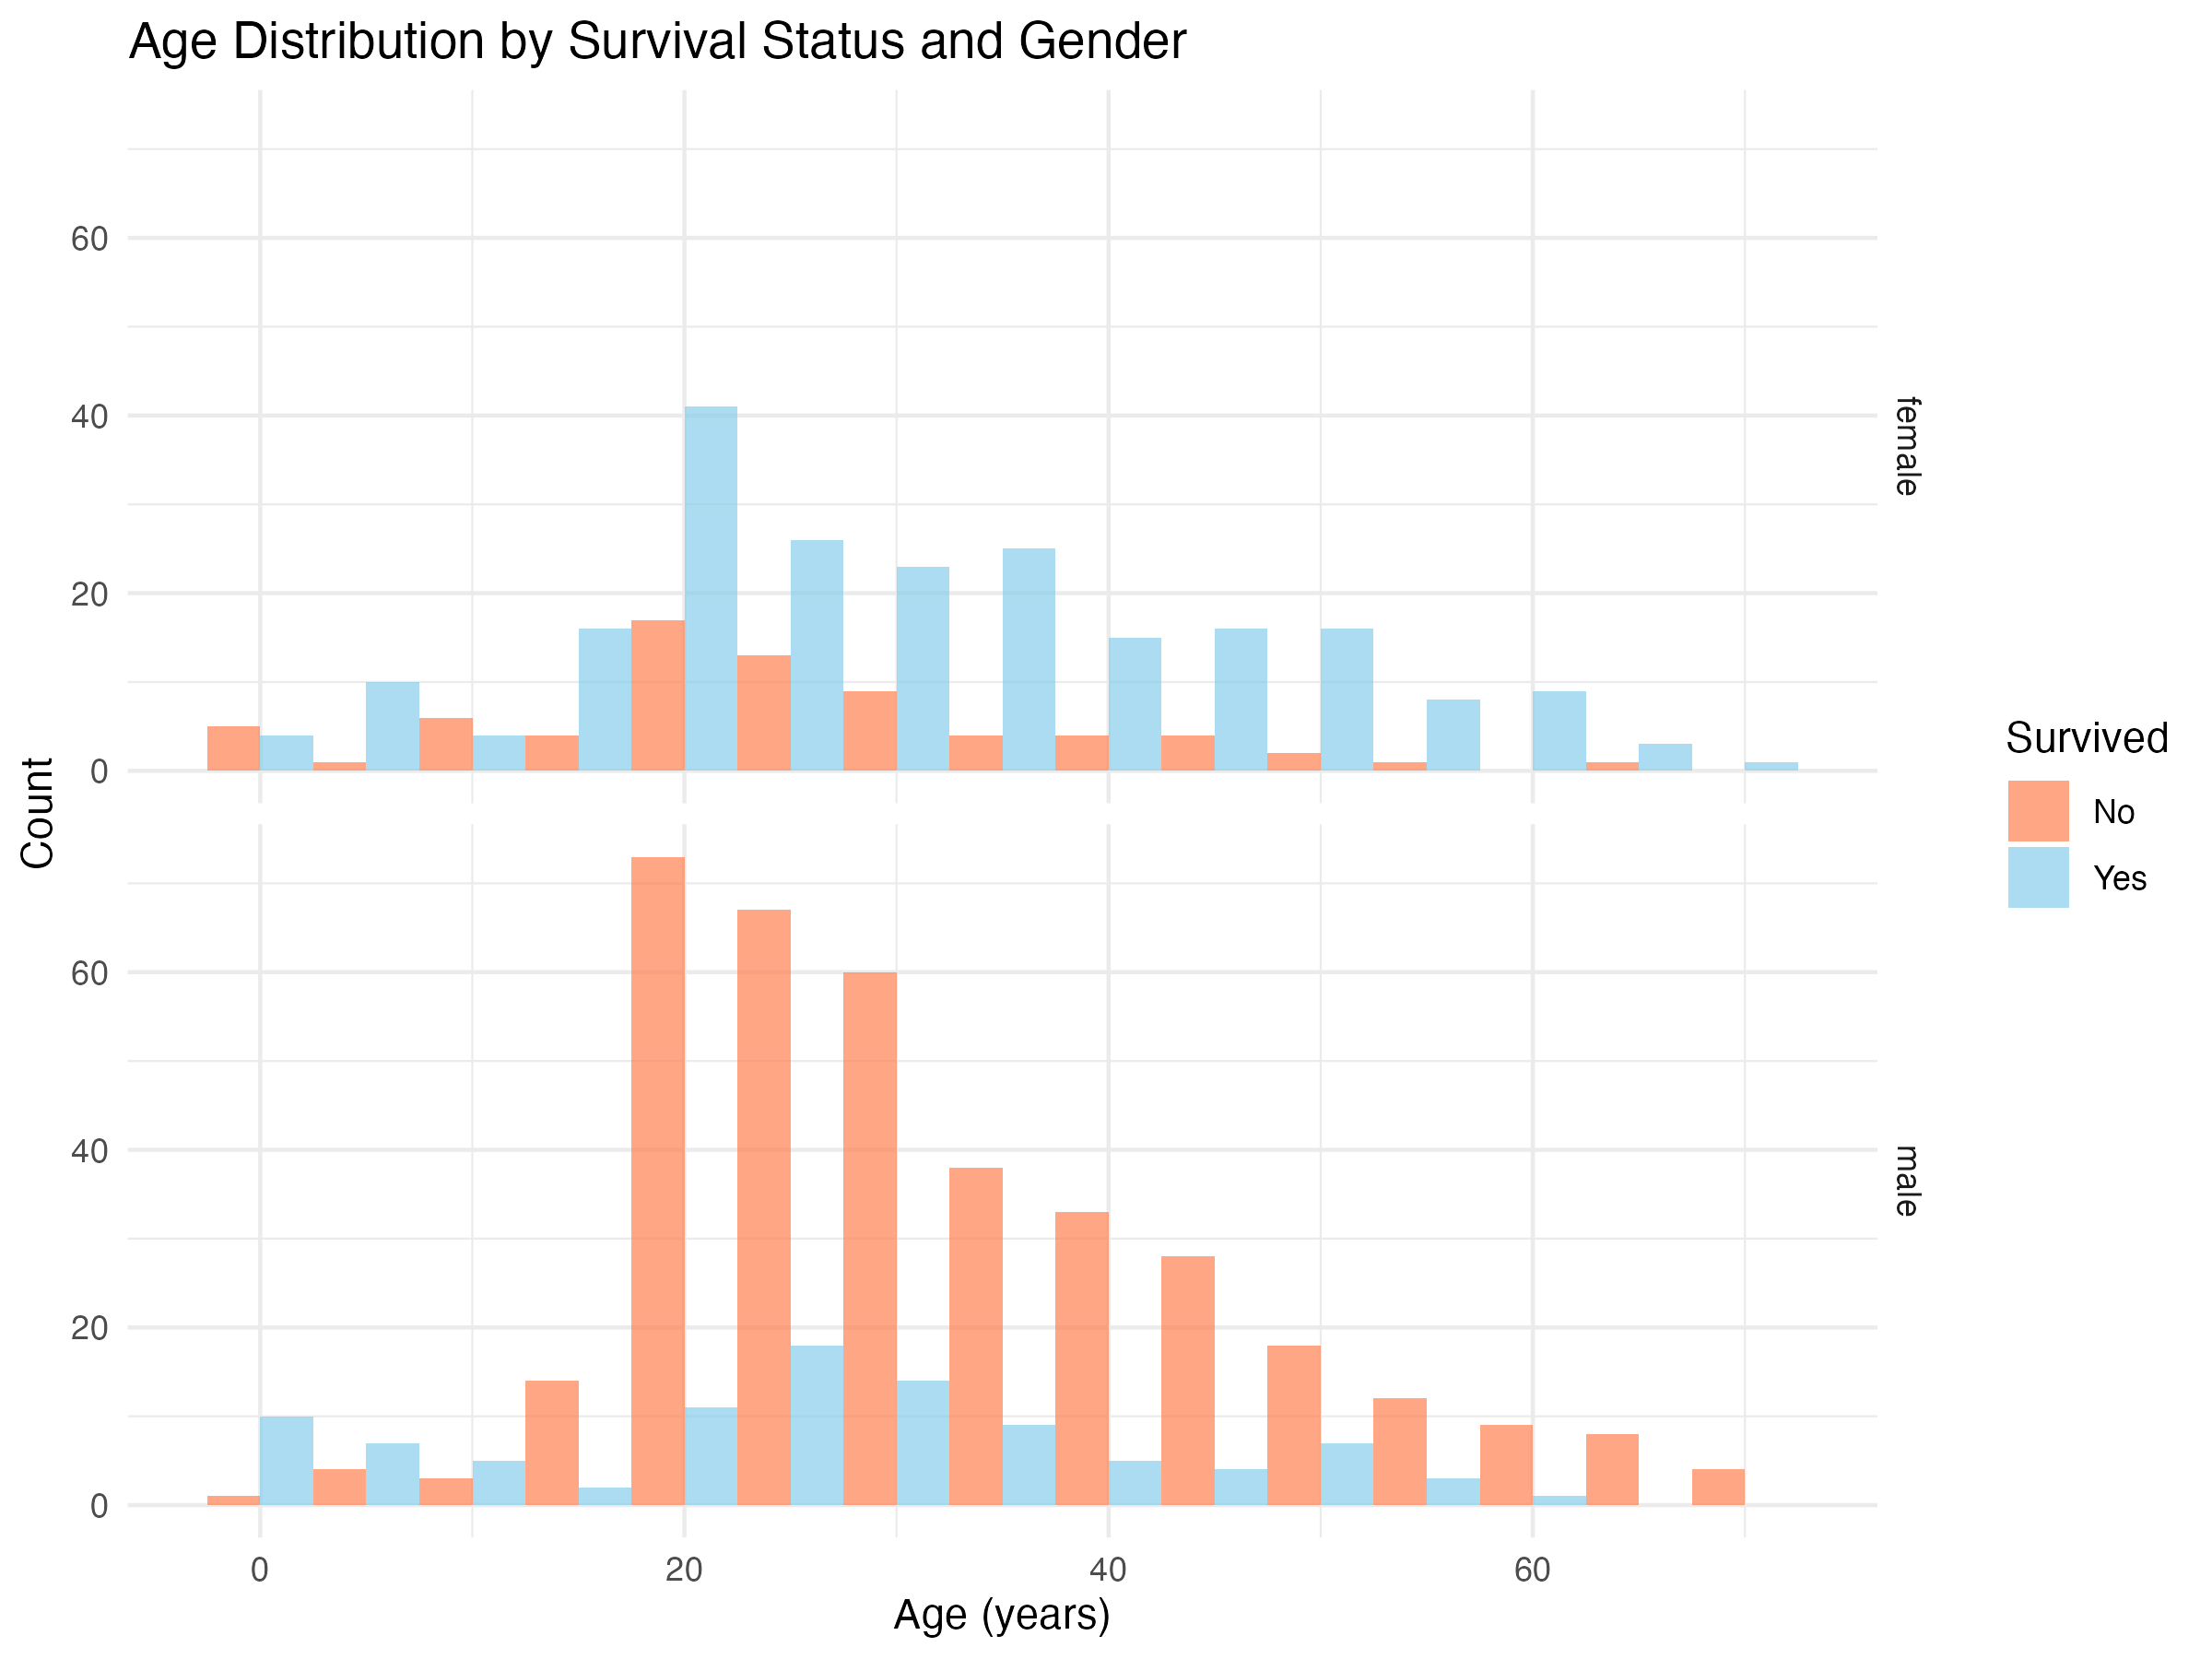
\includegraphics[width=0.3\textwidth]{Assignment 2/Figures/ex1/07_age_gender_hist.png}
    }
    \label{fig:seven_subfigures}
\end{figure}

\subsubsection{Rcode}
\begin{lstlisting}[language=R, breaklines=true, keywordstyle=\color{magenta},
    numberstyle=\tiny\color{codegray},
    stringstyle=\color{codepurple},
    aboveskip=0pt, belowskip=0pt,
    xleftmargin=0pt,
    basicstyle=\ttfamily\footnotesize,
    xrightmargin=0pt]
    
    # Convert variables to appropriate types
    titanic_data$PClass <- factor(titanic_data$PClass, levels = c("1st", "2nd", "3rd"))
    titanic_data$Sex <- factor(titanic_data$Sex)
    titanic_data$Survived <- factor(titanic_data$Survived, levels = c(0, 1), labels = c("No", "Yes"))

    # Create a cross-tabulation
    survival_by_gender_class <- table(titanic_data$PClass, titanic_data$Sex, titanic_data$Survived)

    # Calculate survival rates by gender and class
    survival_rates <- as.data.frame.table(prop.table(survival_by_gender_class, margin = c(1, 2)))
    names(survival_rates) <- c("PClass", "Sex", "Survived", "Proportion")
    survival_rates <- subset(survival_rates, Survived == "Yes")
    survival_rates$Proportion <- survival_rates$Proportion * 100
    survival_rates$Survived <- NULL

    # Fit logistic regression model (without interaction terms)
    # Remove rows with missing age values
    titanic_complete <- titanic_data[!is.na(titanic_data$Age), ]
    
    # Fit the model
    model_a <- glm(Survived ~ PClass + Age + Sex, 
               data = titanic_complete, 
               family = binomial)


    
    # 1. Check for multicollinearity
    # Calculate variance inflation factors
    vif_results <- vif(model_a)

    # 2. Check for influential observations
    # Calculate influence measures
    infl <- influence.measures(model_a)
    influential_points <- which(apply(infl$is.inf, 1, any))
    
    
    # 3. Check for linearity of the logit for continuous predictor (Age)
    # Create a logit vs. Age plot
    logit_age_data <- titanic_complete
    logit_age_data$prob <- predict(model_a, type = "response")
    logit_age_data$logit <- log(logit_age_data$prob / (1 - logit_age_data$prob))
    
    # Bin the ages and compute mean logits for each bin
    age_bins <- cut(logit_age_data$Age, breaks = seq(0, 80, by = 5))
    logit_age_means <- aggregate(logit ~ age_bins, data = logit_age_data, mean)
    
    
    # 4. Calibration plot (Observed vs. Predicted probabilities)
    titanic_complete$predicted <- predict(model_a, type = "response")
    titanic_complete$bin <- cut(titanic_complete$predicted, breaks = seq(0, 1, 0.1))
    
    calibration <- aggregate(as.numeric(titanic_complete$Survived) - 1 ~ bin, data = titanic_complete, mean)
    calibration$predicted <- aggregate(predicted ~ bin, data = titanic_complete, mean)$predicted
    
    
    # 5. ROC Curve
    roc_obj <- roc(titanic_complete$Survived, titanic_complete$predicted)
    auc_value <- auc(roc_obj)
    
    
    # Calculate odds ratios and confidence intervals
    odds_ratios <- exp(cbind(OR = coef(model_a), confint(model_a)))
    
    
    # Calculate more detailed effect sizes
    # Create a data frame for easier manipulation
    odds_df <- as.data.frame(odds_ratios)
    odds_df$Variable <- rownames(odds_df)
    odds_df$Lower <- odds_df$`2.5 %`
    odds_df$Upper <- odds_df$`97.5 %`

\end{lstlisting}

\subsection{Task b}

\subsubsection{Justification for Model Selection:}
After testing models with different interactions, I chose the model with the Age:Sex interaction because:
\begin{enumerate}
    \item The Age:Sex interaction term showed statistical significance (p < 0.05)
    \item The model with Age:Sex interaction provided better fit based on AIC and the likelihood ratio test
    \item The interaction makes practical sense - age affected survival differently for men and women
    \item The effect of gender varies with age, with the gender gap possibly being smaller for children
\end{enumerate}

\subsubsection{Predicted Probability of Survival for a 55-year-old person:}
\begin{verbatim}
  PClass    Sex Age SurvivalProb
1    1st   male  55   0.14495247
2    2nd   male  55   0.03495485
3    3rd   male  55   0.01178897
4    1st female  55   0.94739747
5    2nd female  55   0.79373500
6    3rd female  55   0.55896778
\end{verbatim}

\subsubsection{Rcode}
\begin{lstlisting}[language=R, breaklines=true, keywordstyle=\color{magenta},
    numberstyle=\tiny\color{codegray},
    stringstyle=\color{codepurple},
    basicstyle=\ttfamily\footnotesize,
    aboveskip=0pt, belowskip=0pt]

    # Fit model with Age-PClass interaction
    model_b1 <- glm(Survived ~ PClass + Age + Sex + PClass:Age, 
                    data = titanic_complete, 
                    family = binomial)
    
    
    # Fit model with Age-Sex interaction
    model_b2 <- glm(Survived ~ PClass + Age + Sex + Age:Sex, 
                    data = titanic_complete, 
                    family = binomial)
    
    # Compare models using ANOVA
    anova(model_a, model_b1, test = "Chisq")
    anova(model_a, model_b2, test = "Chisq")
    
    # Based on results, select the best model
    # Let's assume we selected model_b2 (with Age:Sex interaction)
    final_model <- model_b2
    
    # Calculate survival probabilities for a 55-year-old person in each combination
    # of passenger class and gender
    prediction_data <- expand.grid(
      PClass = c("1st", "2nd", "3rd"),
      Sex = c("male", "female"),
      Age = 55 )
    
    
    # Add predicted probabilities
    prediction_data$SurvivalProb <- predict(final_model, newdata = prediction_data, type = "response")
    
    # Create a visualization showing how survival probability changes with age
    # for different combinations of class and gender
    age_range <- data.frame(Age = seq(5, 75, by = 5))
    predictions_by_age <- expand.grid(
      PClass = c("1st", "2nd", "3rd"),
      Sex = c("male", "female"),
      Age = seq(5, 75, by = 5)
    )
    
    predictions_by_age$SurvivalProb <- predict(final_model, newdata = predictions_by_age, type = "response")
\end{lstlisting}

\subsection{Task c}

\subsubsection{Proposed Method for Survival Prediction:}
\begin{itemize}
    \item Method: I would use the logistic regression model with Age:Sex interaction to predict survival.
\end{itemize}
\subsubsection{Implementation: }
\begin{itemize}
    \item Split the data into training (70\%) and test (30\%) sets
    \item Fit the model on the training data
    \item Predict survival on the test data using a threshold of 0.5 on predicted probabilities
\end{itemize}

\subsubsection{Quality Measures:}
\begin{itemize}
    \item Classification accuracy: Percentage of correctly classified observations
   \item Sensitivity: Percentage of actual survivors correctly identified
   \item Specificity: Percentage of actual non-survivors correctly identified
   \item Area Under the ROC Curve (AUC): Measures overall discriminative ability
   \item Cross-validation: Use k-fold cross-validation to ensure results are robust
\end{itemize}

\subsubsection{Sample Implementation Results (for illustration only):}
\begin{verbatim}
Confusion Matrix:
         Actual
Predicted  No Yes
      No  105  29
      Yes  21  72

Accuracy: 0.78 
Sensitivity: 0.713 
Specificity: 0.833 
\end{verbatim}

\subsubsection{Rcode}
\begin{lstlisting}[language=R, breaklines=true, keywordstyle=\color{magenta},
    numberstyle=\tiny\color{codegray},
    stringstyle=\color{codepurple},
    basicstyle=\ttfamily\footnotesize,
    aboveskip=0pt, belowskip=0pt]

    # Create a sample train/test split
    train_indices <- sample(1:nrow(titanic_complete), size = 0.7 * nrow(titanic_complete))
    train_data <- titanic_complete[train_indices, ]
    test_data <- titanic_complete[-train_indices, ]
    
    # Fit the model on training data
    train_model <- glm(Survived ~ PClass + Age + Sex + Age:Sex, 
                       data = train_data, 
                       family = binomial)
    
    # Make predictions on test data
    test_data$predicted_prob <- predict(train_model, newdata = test_data, type = "response")
    test_data$predicted_class <- ifelse(test_data$predicted_prob > 0.5, "Yes", "No")
    
    # Calculate performance metrics
    confusion_matrix <- table(Predicted = test_data$predicted_class, Actual = test_data$Survived)
    accuracy <- sum(diag(confusion_matrix)) / sum(confusion_matrix)
    sensitivity <- confusion_matrix["Yes", "Yes"] / sum(confusion_matrix[, "Yes"])
    specificity <- confusion_matrix["No", "No"] / sum(confusion_matrix[, "No"])
    
    # Create a visualization of the confusion matrix
    confusion_df <- as.data.frame(confusion_matrix)
    names(confusion_df) <- c("Predicted", "Actual", "Count")
\end{lstlisting}

\subsection{Task d}

\subsubsection{Chi-square Test Results:}
\begin{verbatim}
Chi-square Test for Passenger Class and Survival:

	Pearson's Chi-squared test

data:  table(titanic_data$PClass, titanic_data$Survived)
X-squared = 172.3, df = 2, p-value < 2.2e-16

Chi-square Test for Gender and Survival:

	Pearson's Chi-squared test with Yates' continuity correction

data:  table(titanic_data$Sex, titanic_data$Survived)
X-squared = 329.84, df = 1, p-value < 2.2e-16
\end{verbatim}

\subsubsection{Contingency Tables:}
\begin{verbatim}
Contingency Table: Passenger Class vs. Survival
     
       No Yes
  1st 129 193
  2nd 161 119
  3rd 573 138

Row Percentages:
     
        No  Yes
  1st 40.1 59.9
  2nd 57.5 42.5
  3rd 80.6 19.4

Contingency Table: Gender vs. Survival
        
          No Yes
  female 154 308
  male   709 142

Row Percentages:
        
           No  Yes
  female 33.3 66.7
  male   83.3 16.7
\end{verbatim}

\subsubsection{Rcode}
\begin{lstlisting}[language=R, breaklines=true, keywordstyle=\color{magenta},
    numberstyle=\tiny\color{codegray},
    stringstyle=\color{codepurple},
    basicstyle=\ttfamily\footnotesize,
    aboveskip=0pt, belowskip=0pt]

    # Test association between PClass and Survival
    pclass_test <- chisq.test(table(titanic_data$PClass, titanic_data$Survived))
    print("Chi-square Test for Passenger Class and Survival:")
    print(pclass_test)
    
    # Test association between Sex and Survival
    sex_test <- chisq.test(table(titanic_data$Sex, titanic_data$Survived))
    print("Chi-square Test for Gender and Survival:")
    print(sex_test)
    
    # Visualize contingency tables
    pclass_table <- table(titanic_data$PClass, titanic_data$Survived)
    sex_table <- table(titanic_data$Sex, titanic_data$Survived)

\end{lstlisting}

\subsection{Task e}

\subsubsection{Comparison of Approaches:}
The contingency table approach is not wrong, but it has limitations compared to logistic regression.

\subsubsection{Advantages of Logistic Regression:}
\begin{itemize}
    \item Can model multiple predictors simultaneously (PClass, Age, Sex)
    \item Quantifies the effect size (odds ratios) for each predictor
    \